%!TEX root = ../thesis.tex
\chapter{Discussion}
\label{chapter_conclusion}

\section{Restatement of Contributions}
In this dissertation,

% How to design tutorial systems appropriately for different situations
% * level of expertise of instructor, learner
% * what are you trying to make easier?

\section{Remaining Challenges and Future Directions}

\subsection{Non-Linear Tutorials}
branching

\subsection{Emerging Instructional Space}

Augmented and virtual reality systems are becoming available to end users via affordable forms. However, designing AR and VR experiences extremely requires expertise and efforts. As devices offer personalized effects supported by sensing and input techniques, we need new authoring tools that focus on delivering story-centric experiences. Tools should also enable both professionals and amateurs to create and iterate designs efficiently in an immersive 3D world. ...research what future AR and VR creation tools would look like with new authoring processes.

\begin{figure*}[ht!]
  \centering
\begin{tabular}{cc}
  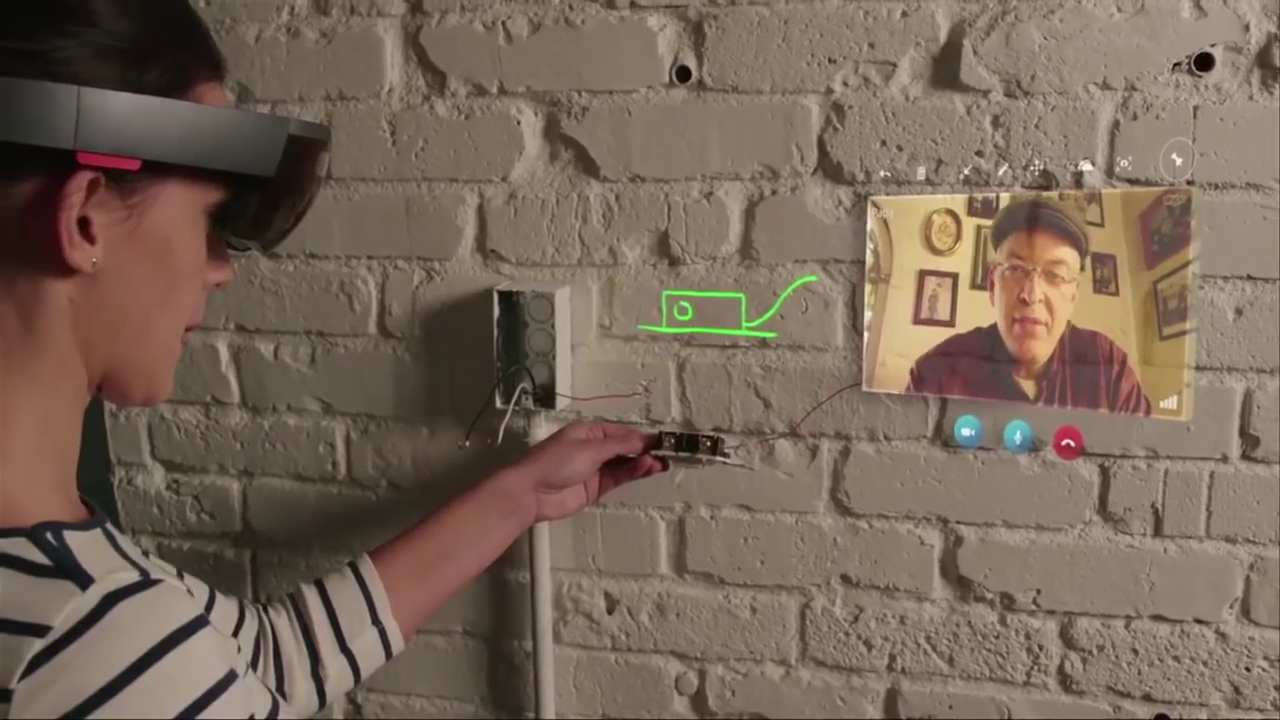
\includegraphics[width=0.4\textwidth]{\conclusion/fig/ar/hololens_fix1} &
  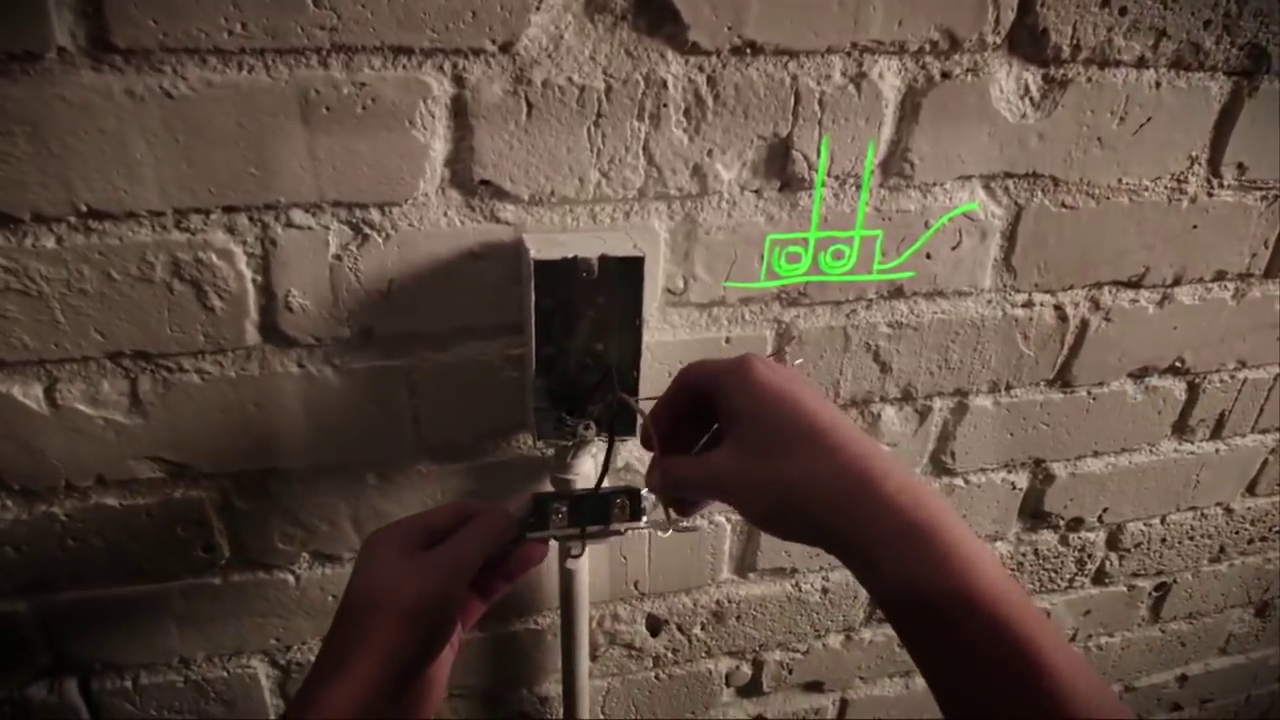
\includegraphics[width=0.4\textwidth]{\conclusion/fig/ar/hololens_fix2} \\
\multicolumn{2}{c}{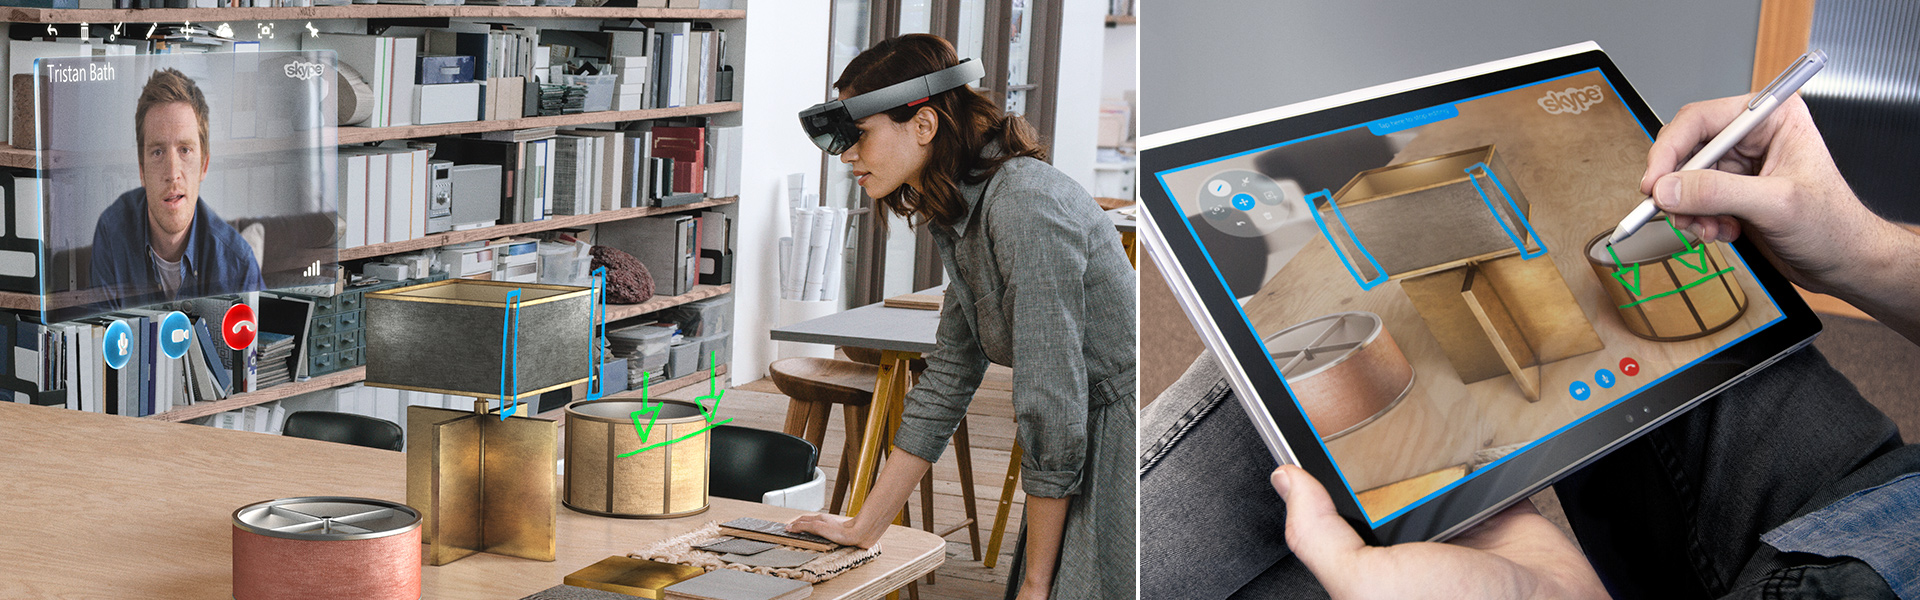
\includegraphics[width=0.82\textwidth]{\conclusion/fig/ar/hololens_skype} }
\end{tabular}
\caption{
  Microsoft's HoloLens~\cite{MicrosoftHoloLensSkype} has introduced an Augmented Reality application on providing real-time physical instructions from a remote instructor.
}
\end{figure*}

\section{Conclusion}
Instructions...
